\documentclass[11pt]{article}

\usepackage[utf8]{inputenc}
\usepackage[T1]{fontenc}
\usepackage[margin=1in]{geometry}
\usepackage{amsmath}
\usepackage{amssymb}
\usepackage{graphicx}
\graphicspath{{../}}
\usepackage{hyperref}
\usepackage{xcolor}
\usepackage{enumitem}
\usepackage{float}
\usepackage{tikz}
\usetikzlibrary{arrows.meta, positioning}

\hypersetup{
  colorlinks=true,
  linkcolor=blue!50!black,
  citecolor=blue!50!black,
  urlcolor=blue!50!black,
  pdftitle={What Likelihood Means},
  pdfauthor={Warith Harchaoui}
}

\usepackage[round]{natbib}
\bibliographystyle{plainnat}

\newcommand{\code}[1]{\texttt{#1}}

\title{What Likelihood Means: \\ From a Raw Product to a Bounded, Comparable Score}
\author{Warith Harchaoui}
\date{Summer 2026}

\begin{document}
\maketitle

\begin{abstract}
This note derives, from first principles, a single idea used across
statistics, information theory and machine learning: read likelihood not
as the raw product every textbook opens with, but as an exponentiated
\emph{average} log-density, $L := \exp(\mathbb E[\ln p])$. That
reformulation is unusual: almost no standard reference defines
likelihood this way. This note explains precisely why it earns its
keep: an exact identity back to the textbook product, a direct
information-theoretic reading (Jensen's inequality, Shannon entropy, a
temperature-indexed refinement borrowed from equilibrium statistical
mechanics), two classical asymptotic results (Cram\'er's large
deviations and Wald's martingale) that describe exactly this quantity's
long-run behavior, and a precise account of $L$ as a statistical
estimator, bias and variance included, together with a proof that the
raw product it replaces is not an estimator of anything fixed at all.
Two worked instantiations, a categorical classification model and a
regression model under Gaussian noise, show the same construction
landing on the reciprocal of a familiar error measure in both cases,
perplexity in the first, root-mean-square error in the second.
\code{elbow-helper}'s own mathematics note, \code{ELBOW-en.tex}, builds
its Gaussian model-selection criteria (BIC, $\mathrm{mBIC}$, ICL) on top
of the foundation derived here rather than re-deriving it. Citations
follow the same evidence-marking convention as \code{ELBOW-en.tex}: each
claim states whether it is a verified citation, a citation reported
through a secondary source, or this note's own construction.
\end{abstract}

\clearpage

\tableofcontents

\clearpage

\section{The notion}
\label{sec:notion}

Data here means $n$ pairs $(x_i, y_i)$, an input $x_i$ paired with an
outcome $y_i$: a covariate driving a prediction, a position driving a
curve's height, or nothing at all, $x_i$ simply absent, for a model that
only ever describes $y_i$ on its own. A single graphical model covers
every case this note uses, $\theta$ and $x_i$ feeding a conditional
density that generates $y_i$:

\begin{center}
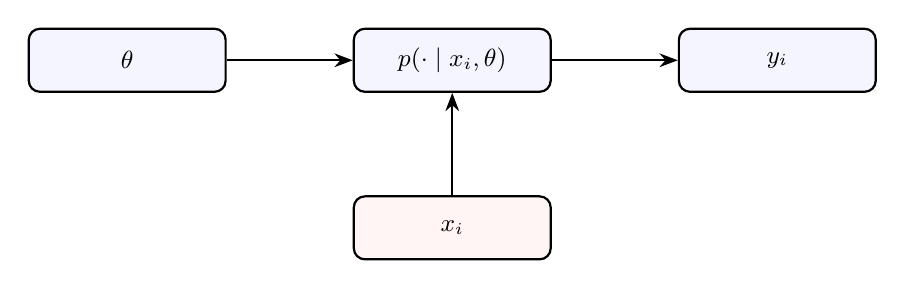
\begin{tikzpicture}[
  node distance=13mm and 16mm,
  box/.style={draw, rounded corners, minimum height=8mm, minimum width=25mm,
    align=center, font=\small, fill=blue!4},
  ->, >=Stealth, thick
]
\node[box] (theta) {$\theta$};
\node[box, right=of theta] (dens) {$p(\cdot \mid x_i,\theta)$};
\node[box, right=of dens] (y) {$y_i$};
\node[box, below=of dens, fill=red!4] (x) {$x_i$};
\draw (theta) -- (dens);
\draw (dens) -- (y);
\draw (x) -- (dens);
\end{tikzpicture}
\end{center}

\emph{Likelihood} names the joint density of the observed outcomes,
read as a function of the parameter rather than the data:
$L_{\text{raw}}(\theta) := \prod_{i=1}^n p(y_i \mid x_i, \theta)$, a
plain product of $n$ terms, one per observation. This is the definition
every standard treatment opens with, Bishop's among the clearest
\citep{bishop2006prml}. It is also the exact quantity a Bayes factor or a
Neyman-Pearson likelihood-ratio test compares directly. Left as a raw
product, though, it is a poor building block for a bounded score: $n$
densities multiplied together either shrink toward zero or explode as
$n$ itself grows, so $L_{\text{raw}}$ on $40$ points and $L_{\text{raw}}$
on $4{,}000$ points are not numbers a single threshold could ever
compare; the raw product carries the sample size baked into its scale.

This note departs from that convention immediately and says so plainly
rather than leaving the departure implicit inside a formula: it takes
likelihood \emph{per observation} from the outset, an exponentiated
\emph{average} log-density rather than a raw product,
$$L := \exp\!\big(\mathbb E[\ln p]\big) = L_{\text{raw}}^{\,1/n},$$
the geometric mean of the $n$ individual densities, exactly the $n$-th
root of $L_{\text{raw}}$, never a different number, only a different
form of the same one. Almost no standard reference defines likelihood
this way. The reason is not stylistic: dividing the exponent's sum by
$n$ before re-exponentiating is exactly what turns an extensive
quantity, one whose scale depends on sample size, into an intensive
one, whose scale does not, the same move information theory makes when
it works with \emph{perplexity}, an exponentiated \emph{average}
log-probability, rather than a raw joint one (made literal in
Section~\ref{sec:worked}).

\section{What the number means}
\label{sec:meaning}

Before any asymptotic machinery, $L$ has a direct reading worth sitting
with. By Jensen's inequality, since $\ln$ is concave, $L = \exp(\mathbb
E[\ln p]) \le \mathbb E[p]$ always: the geometric mean this note works
with never exceeds the arithmetic mean of the same densities, with
equality only when $p$ is constant across observations.

For a discrete $p$ over $K$ outcomes, take the expectation under $p$
itself rather than under data: $\exp(\mathbb E_{y \sim p}[\ln p_y]) =
\exp(-H(p))$, Shannon's entropy \citep{mackay2003information} read as a
probability rather than a bit count. This sits in $[1/K, 1]$: equal to
$1/K$ when $p$ is uniform over the $K$ outcomes, rising to $1$ as $p$
concentrates on one of them. Read this way, $\exp(-H(p))$ is a typical,
or effective, probability. Its reciprocal $\exp(H(p))$ is the effective
number of plausible outcomes: $\exp(H(p)) \approx 4$ means about as
uncertain as a fair guess among four.

\textbf{A temperature reading.} That bound has a one-parameter
refinement worth making precise rather than merely evocative. For
$\beta > 0$, define the power-tilted family $p_\beta(y) := p(y)^\beta /
Z(\beta)$, $Z(\beta) := \int p(y)^\beta\,dy$ (or $\sum_y p(y)^\beta$ in
the discrete case): a genuine exponential family, with $\beta$ playing
the role Gibbs assigns to inverse temperature against the ``energy''
$-\ln p(y)$. This is exactly the object the large-deviations
statistical-mechanics dictionary describes: $\ln Z(\beta)$ is a scaled
free energy, $\beta$ its inverse temperature, and the Legendre-transform
relationship Section~\ref{sec:why}'s Cram\'er argument uses for the rate
function is, term for term, the one relating free energy and entropy in
equilibrium statistical mechanics \citep{touchette2009}. Differentiating
at $\beta=1$, where $p_\beta = p$, recovers $L$ itself: $\frac{d}{d\beta}
\ln Z(\beta)\big|_{\beta=1} = \mathbb E_p[\ln p] = \ln L$, so $L$ is one
derivative of a free energy, evaluated at one specific temperature. The
Shannon entropy above is itself the $\beta \to 1$ limit of the R\'enyi
entropy $H_\beta(p) := \ln Z(\beta)/(1-\beta)$, a standard fact checked
directly from the definitions above.

The two extremes of $\beta$ read exactly like the two extremes of
temperature, made precise rather than left as image. As $\beta \to
0^+$, hot and maximally agitated, $p_\beta$ flattens toward uniform over
$p$'s support regardless of what $p$ itself looked like: $Z(\beta) \to
K$ in the $K$-category case, so $\exp(-H_\beta(p)) \to 1/K$, exactly the
floor derived above. As $\beta \to \infty$, cold and frozen, $p_\beta$
collapses onto $p$'s own mode: $\exp(-H_\beta(p)) \to \max_k p_k$, the
probability of the single most likely category, a tighter, $p$-dependent
ceiling than the loose upper bound of $1$ (reached only in the
degenerate limit where $p$ itself is already a point mass). Verified
numerically on $p = (0.5, 0.3, 0.15, 0.05)$: $\exp(-H_\beta(p))$ moves
from $0.25 = 1/4$ at $\beta \to 0$ to $0.5 = \max_k p_k$ at $\beta \to
\infty$, monotonically, passing through $\exp(-H(p)) \approx 0.32$ at
$\beta = 1$. Water's own two familiar extremes at atmospheric pressure,
freezing at $0\,^\circ\mathrm C$ and boiling at $100\,^\circ\mathrm C$,
are a physical illustration of exactly this shape, a fixed system swept
from an ordered, low-entropy phase to a disordered, high-entropy one as
an inverse-temperature-like parameter crosses its range, not a
numerical correspondence: nothing here claims $\beta = 0$ or $\beta =
\infty$ literally sit at those two Celsius values, only that the
qualitative mechanism and its exact Legendre-transform bookkeeping are
the ones equilibrium statistical mechanics already worked out.

\begin{figure}[H]
\centering
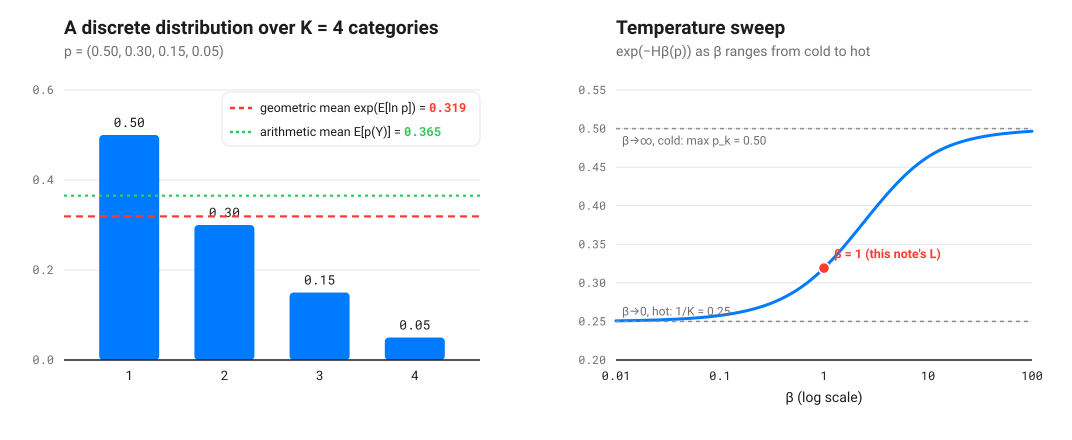
\includegraphics[width=\textwidth]{figures/temperature_sweep_en.png}
\caption{Left: the bar chart above, $p = (0.5, 0.3, 0.15, 0.05)$, with
its geometric mean $\exp(\mathbb E[\ln p]) \approx 0.319$ and arithmetic
mean $\mathbb E[p(Y)] \approx 0.365$ marked, Jensen's inequality made
visible as two horizontal lines rather than left as a bare formula.
Right: $\exp(-H_\beta(p))$ swept across $\beta$, hot on the left, cold
on the right, moving monotonically from the floor $1/K = 0.25$ to the
ceiling $\max_k p_k = 0.5$, with $\beta = 1$, this note's own $L$,
marked where it sits along that path.}
\label{fig:temperature}
\end{figure}

\section{Why an average, not a sum: large deviations and martingales}
\label{sec:why}

Two classical results say this is not just a convenient rescaling. Write
$Z_i := \ln p(y_i \mid x_i, \theta)$ for the per-observation log-density,
so $L = \exp\big(\frac1n\sum_i Z_i\big)$, an exponentiated sample mean.
First, the exact relation this buys back to $L_{\text{raw}}$: $L^n =
\exp\big(\sum_i Z_i\big) = \prod_i p(y_i \mid x_i, \theta) =
L_{\text{raw}}(\theta)$. Taking the $n$-th root and re-exponentiating an
average does not lose information relative to the raw product; it is the
same number, an $n$-th root away, now expressed in the one form whose
large-sample behavior is understood.

Cram\'er's theorem \citep{cramer1938}, the founding result of
large-deviations theory, says an i.i.d.\ sample mean like $\frac1n\sum_i
Z_i$ does more than converge to $\mathbb E[Z]$, the law of large
numbers' guarantee; the probability that it strays from that limit by
more than any fixed amount decays exponentially in $n$, at a rate set by
a convex rate function, the Legendre transform of $Z$'s cumulant
generating function. Working with the average first, rather than the raw
product $L^n$ it is one root away from, is what exposes that exponential
structure instead of burying it inside an already-multiplied number.

Chernoff \citep{chernoff1952} specializes exactly this machinery to
deciding between two densities $p_0, p_1$ from $n$ i.i.d.\ draws, in the
symmetric setting where both hypotheses carry a prior and a single test
minimizes the total (Bayes) probability of error rather than one error
type at a fixed level of the other: the best total error probability any
such test can achieve decays as $\exp(-n\,C(p_0,p_1))$, where the
\emph{Chernoff information} $C(p_0,p_1) := -\min_{\lambda \in [0,1]} \ln
\int p_0^\lambda p_1^{1-\lambda}$ is, structurally, one more
exponentiated average of a log, this time an integral over the sample
space rather than a mean over observations. This is a different question
from the one the Chernoff-Stein lemma answers, fixing one error type's
probability and asking how fast the other can be driven down, which
lands on the Kullback-Leibler divergence rather than the Chernoff
information; the two results are often confused precisely because both
carry Chernoff's name.

The same running product has a second, complementary life as a
\emph{process} rather than a single number. Define the likelihood-ratio
process $\Lambda_t := \prod_{i=1}^t p_1(y_i)/p_0(y_i) =
\exp\big(\sum_{i=1}^t \ln[p_1(y_i)/p_0(y_i)]\big)$ over the first $t$
observations. Under $p_0$, $\Lambda_t$ is a nonnegative martingale,
$\mathbb E_{p_0}[\Lambda_t \mid \mathcal F_{t-1}] = \Lambda_{t-1}$, the
fact Wald \citep{wald1945} built the Sequential Probability Ratio Test
on: a threshold crossed by $\Lambda_t$ at a data-dependent stopping time
still controls the test's error rate, by the optional stopping theorem,
the guarantee a fixed-$n$ test gets automatically and a naively-stopped
one does not. That guarantee needs two fully specified densities $p_0$
and $p_1$, though, a requirement not every sequential problem can meet;
\code{elbow-helper}'s own sequential test (\code{ELBOW-en.tex}, the
sequential-test section, \code{sec:fwer}) is exactly such a case, its
alternative at each step a composite, best-fitting extra breakpoint
rather than a second fixed density, which is why it calibrates against a
permutation null instead of Wald's classical martingale bound.

\textbf{Two different questions about $L$ as an estimator.} Everything
computed so far, $L$ included, comes from a finite sample, so two
distinct questions are worth separating cleanly rather than letting
either one hide inside the other. First: is the sample-based $L$ this
note computes on $n$ real observations a good estimator of the
population value it converges to as $n \to \infty$? Second: does the
raw, un-rooted product $L_{\text{raw}}$, this note's own $L$ before the
$n$-th root is taken, estimate that same population value at all? Fix
the target first. Let $(X_1,Y_1),\dots,(X_n,Y_n)$ be drawn i.i.d.\ from
the true joint data distribution $q$. Let $p_\theta$ be a candidate
model for $p(y \mid x)$. As $n \to \infty$, this note's own $L$ is built
to converge to one fixed number,
$$L_\infty := \exp(\mu_Z), \qquad \mu_Z := \mathbb E_q\big[\ln
p_\theta(Y \mid X)\big],$$
not a random quantity: $\mu_Z$ is an ordinary expectation under the true
$q$, a single number once $p_\theta$ and $q$ are fixed. Two different
sample-based quantities can now be compared against that one target.

The first is this note's own $L$, computed on $n$ observed pairs:
$\hat L_n := \exp(\bar Z_n)$, $\bar Z_n := \frac1n\sum_i Z_i$, $Z_i :=
\ln p_\theta(Y_i \mid X_i)$. $\bar Z_n$ is exactly unbiased for $\mu_Z$,
so $\hat L_n$ is a genuine estimator of $L_\infty$, though not an
unbiased one: $\exp$ is convex, so Jensen's inequality, the same one
Section~\ref{sec:meaning} used to bound $L$ itself, gives $\mathbb
E[\hat L_n] \ge L_\infty$ always. The delta method makes the size of
that upward bias explicit,
$$\mathbb E[\hat L_n] = L_\infty\Big(1 + \frac{\sigma_Z^2}{2n} +
O(n^{-2})\Big), \qquad \mathrm{Var}[\hat L_n] = L_\infty^2\,
\frac{\sigma_Z^2}{n} + O(n^{-2}), \qquad \sigma_Z^2 :=
\mathrm{Var}_q[Z],$$
both vanishing as $n \to \infty$: $\hat L_n$ is consistent, in fact
$\sqrt n$-consistent and asymptotically normal, $\sqrt n(\hat L_n -
L_\infty) \to \mathcal N(0, L_\infty^2\sigma_Z^2)$ in distribution, its
bias shrinking at the same $O(1/n)$ rate as its variance. (Monte Carlo
simulation with a well-specified $p_\theta = q$, $10^5$ replicates per
sample size $n \in \{5,\dots,1000\}$, matches both formulas closely at
every $n$ tried, this note's own verification rather than a claim
requiring a citation.)

The second candidate is the raw product this note opened by rejecting,
$L_{\text{raw}} := \prod_i p_\theta(Y_i \mid X_i) = \hat L_n^{\,n} =
\exp(n\bar Z_n)$. Is it also an estimator of $L_\infty$? Its expectation
answers the question directly:
$$\mathbb E[L_{\text{raw}}] = \big(\mathbb E_q[e^Z]\big)^n =
\exp\!\big(n\,\Lambda(1)\big), \qquad \Lambda(u) := \ln \mathbb
E_q[e^{uZ}],$$
where $\Lambda$ is exactly the cumulant generating function Cram\'er's
argument above is built from. For $\mathbb E[L_{\text{raw}}]$ to
converge to $L_\infty$, or to anything fixed at all, $\Lambda(1)$ would
need to equal $0$ exactly, a knife-edge condition with no reason to
hold for a generic $p_\theta$. Absent it, $\mathbb E[L_{\text{raw}}]$
decays to $0$ or explodes to $\infty$ exponentially fast in $n$.
$L_{\text{raw}}$ is not a biased or noisy estimator of $L_\infty$: it is
not an estimator of it at all, the precise, quantitative version of
Section~\ref{sec:notion}'s opening observation that $L_{\text{raw}}$ on
$40$ points and on $4{,}000$ points are not numbers a single threshold
could ever compare.

\section{Two worked instantiations}
\label{sec:worked}

The same construction, an exponentiated average log-density, lands on
the reciprocal of a familiar error measure in both of the settings
machine learning most often fits: a categorical classification model and
a regression model under Gaussian noise.

\subsection{Classification}
\label{sec:classification}

A classifier's generative model is the same graphical model as
Section~\ref{sec:notion}'s, specialized to a categorical outcome: $x_i$
and $\theta$ set a probability vector over $K$ classes, and $y_i$ is
drawn from it.

\begin{center}
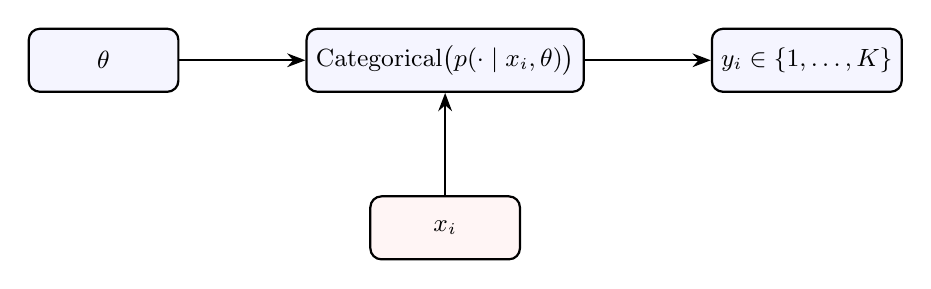
\begin{tikzpicture}[
  node distance=13mm and 16mm,
  box/.style={draw, rounded corners, minimum height=8mm, minimum width=19mm,
    align=center, font=\small, fill=blue!4},
  ->, >=Stealth, thick
]
\node[box] (theta) {$\theta$};
\node[box, right=of theta] (dens) {$\mathrm{Categorical}\big(p(\cdot \mid x_i,\theta)\big)$};
\node[box, right=of dens] (y) {$y_i \in \{1,\dots,K\}$};
\node[box, below=of dens, fill=red!4] (x) {$x_i$};
\draw (theta) -- (dens);
\draw (dens) -- (y);
\draw (x) -- (dens);
\end{tikzpicture}
\end{center}

If $Y$ is the true class and a model predicts $p(Y \mid X)$, $\exp(\mathbb
E_{(X,Y)}[\ln p(Y \mid X)]) = \exp(-\mathrm{CE})$ is exactly the
geometric-mean probability the model assigns to the correct class, a
reading no raw cross-entropy in nats offers directly. A cross-entropy of
$0.693$ nats, $\ln 2$, becomes $\exp(-0.693) \approx 0.5$: a model about
as confident, on the correct class, as a coin flip. Equivalently,
$\exp(\mathrm{CE})$ is the \emph{perplexity} the model assigns to the
true class, the effective number of classes it is choosing among as far
as its confidence is concerned; a perplexity near $1$ is a confident,
well-calibrated model, a perplexity near $K$ (the class count) is no
better than guessing uniformly.

Take the $p = (0.5, 0.3, 0.15, 0.05)$ example Figure~\ref{fig:temperature}
already plotted, now read as one model's predicted probabilities for one
example, class $1$ the true label. The model's cross-entropy on that
single example is $\mathrm{CE} = -\ln p_1 = -\ln 0.5 \approx 0.693$
nats, exactly the coin-flip case above: the model assigns the true
class only even odds, even though it is the single most likely class
under its own prediction. Averaged over many examples rather than read
off one, the same $\exp(-\mathrm{CE})$ becomes the geometric-mean
probability the model assigns to whichever class turns out true each
time. Figure~\ref{fig:temperature}'s right-hand panel is exactly that
averaging machine turned into a dial: $\beta = 1$ is the ordinary,
untilted cross-entropy read above, $\beta \to 0$ softens every
prediction toward uniform confidence over all $K$ classes regardless of
the model's own opinion, while $\beta \to \infty$ hardens every
prediction toward its single most likely class, a temperature knob
turning a probabilistic classifier into something closer to a bare
arg\,max as it cools.

Figure~\ref{fig:classification} takes this from one hand-picked example
to a genuine simulation: $45$ points drawn from $3$ overlapping classes,
each assigned a probability for its own true class by a simple
distance-to-centroid softmax model. Some points sit deep inside their
own class's territory and score high; others sit near a boundary between
two classes and score low, the model genuinely unsure which label is
right. $L$ is the geometric mean of all $45$ of those individual
probabilities, not an arbitrary summary of them: the right-hand panel
sorts them low to high and marks exactly where that geometric mean
falls, visibly closer to the crowd of low scores than an arithmetic mean
would sit, the same pull toward the worst cases Jensen's inequality
already predicted.

\begin{figure}[H]
\centering
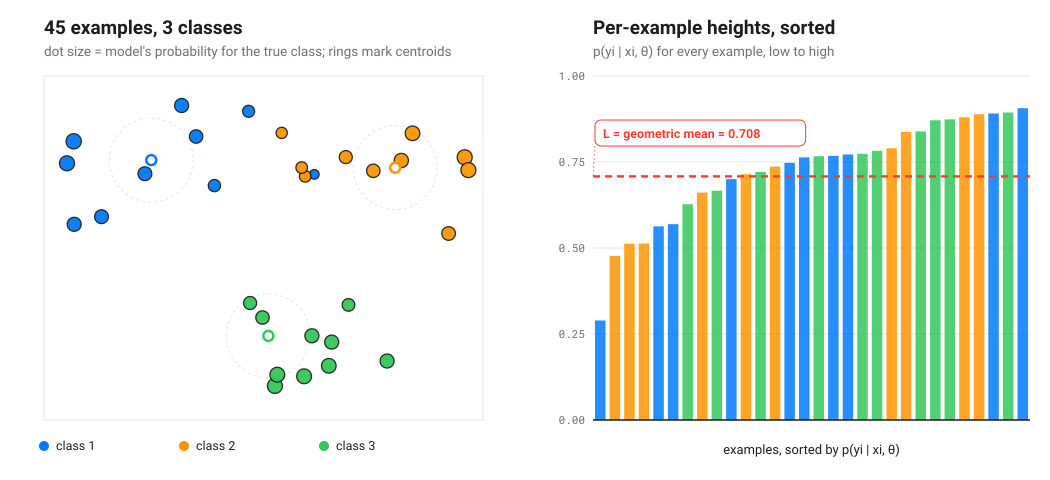
\includegraphics[width=\textwidth]{figures/classification_density_en.png}
\caption{Left: $45$ simulated examples from $3$ overlapping classes
(dashed rings mark the generating centroids), dot size showing the
model's probability for each example's own true class, small near a
class boundary, large deep inside a class's territory. Right: those same
$45$ probabilities sorted from low to high, with their geometric mean,
this note's $L$, marked.}
\label{fig:classification}
\end{figure}

A single scalar, though, whether $\mathrm{CE}$, $\exp(-\mathrm{CE})$, or
a perplexity, only ever answers ``how confident, on average'', never
``how often actually right''. A model can be confidently wrong,
assigning high probability to an incorrect class. $\mathrm{CE}$
penalizes exactly that overconfidence more harshly than a small, honest
uncertainty would be penalized, the same asymmetry a proper scoring rule
is built to have: guessing $99\%$ on a class that turns out false costs
far more in nats than guessing $60\%$ ever would. That asymmetry, not
merely the average confidence level, is why cross-entropy rather than
raw classification accuracy is the quantity fit by gradient descent in
essentially every modern classifier.

\subsection{Regression under Gaussian noise}
\label{sec:regression}

Let $y_i = f(x_i;\theta) + \varepsilon_i$ with $\varepsilon_i$ i.i.d.\
$\mathcal N(0,\sigma^2)$, $f$ any regression function and $\theta$ its
parameters, the generic conditional density of Section~\ref{sec:notion}
specialized to one particular family:

\begin{center}
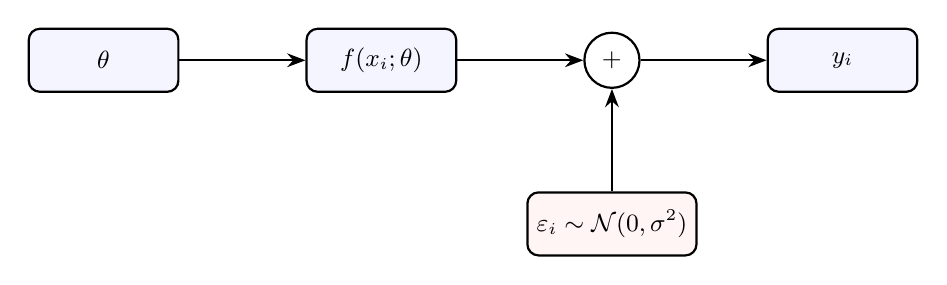
\begin{tikzpicture}[
  node distance=13mm and 16mm,
  box/.style={draw, rounded corners, minimum height=8mm, minimum width=19mm,
    align=center, font=\small, fill=blue!4},
  sum/.style={draw, circle, minimum size=7mm, inner sep=0pt, font=\small},
  ->, >=Stealth, thick
]
\node[box] (theta) {$\theta$};
\node[box, right=of theta] (f) {$f(x_i;\theta)$};
\node[sum, right=of f] (sum) {$+$};
\node[box, right=of sum] (y) {$y_i$};
\node[box, below=of sum, fill=red!4] (eps) {$\varepsilon_i \sim \mathcal N(0,\sigma^2)$};
\draw (theta) -- (f);
\draw (f) -- (sum);
\draw (sum) -- (y);
\draw (eps) -- (sum);
\end{tikzpicture}
\end{center}

\begin{equation}
p(y_i \mid x_i, \theta) = (2\pi\sigma^2)^{-1/2}
\exp\!\left(-\frac{(y_i - f(x_i;\theta))^2}{2\sigma^2}\right)
\end{equation}

so that, writing $\mathrm{MSE}(\theta) := \frac1n\sum_i (y_i -
f(x_i;\theta))^2$,

\begin{equation}
L(\theta,\sigma^2) = (2\pi\sigma^2)^{-1/2}\exp\!\left(-\frac{\mathrm{MSE}(\theta)}{2\sigma^2}\right).
\end{equation}

Figure~\ref{fig:regression} draws this density literally rather than
only in symbols: a small bell curve at a few chosen $x$ positions, each
one the conditional density $p(\cdot \mid x_i,\theta)$ turned on its
side, its width set by $\sigma$ and its center riding along the fitted
line. The marked dot on each bell is that curve's own height at the
point actually observed, $p(y_i \mid x_i,\theta)$, tall where the fit
lands close to the data, short where it does not. $L$ is nothing more
than the geometric mean of those heights taken over every observation,
not only the four marked ones, the exact continuous counterpart of
Figure~\ref{fig:classification}'s sorted bars: a curve fit closely
almost everywhere posts mostly tall heights and a large $L$, a curve
that wanders posts some short ones and pulls the geometric mean down,
one bad miss doing more damage to a geometric mean than to an arithmetic
one, the same asymmetry Section~\ref{sec:meaning}'s Jensen bound already
flagged.

At the maximum-likelihood variance $\hat\sigma^2 = \mathrm{MSE}(\theta)$,

\begin{equation}
\exp(\mathbb E[\ln p]) = \frac{1}{\sqrt{2\pi e}\,\sqrt{\mathrm{MSE}(\theta)}},
\end{equation}

the reciprocal of the root-mean-square error up to a universal constant
$\sqrt{2\pi e}$, the exact continuous counterpart of
Section~\ref{sec:classification}'s reciprocal-perplexity reading: in
both cases $\exp(\mathbb E[\ln p])$ is the reciprocal of an error
measure native to the prediction task, perplexity for a categorical one,
root-mean-square error for a continuous one. This is no coincidence.
Writing $\ell := \ln L$ and, following the convention information
criteria use, $\mathrm{PPL} := \exp(-2\ell)$, the identity $\exp(\mathbb
E[\ln p]) = 1/\sqrt{\mathrm{PPL}}$ holds in general, Gaussian or not, a
direct consequence of the two definitions rather than a property
specific to either worked case. \code{elbow-helper}'s own
\code{ELBOW-en.tex} takes this instantiation further: $f$ there ranges
over single lines, broken lines and $k$-segment piecewise lines.
$\mathrm{PPL}$ is turned into a genuinely bounded, worst-case-anchored
score rather than left as a bare reciprocal-RMSE reading.

\begin{figure}[H]
\centering
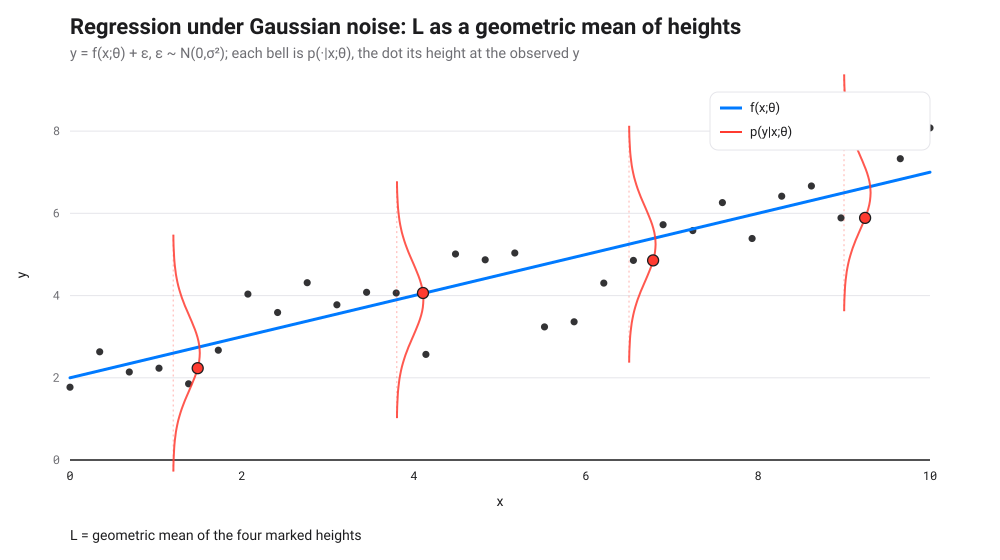
\includegraphics[width=\textwidth]{figures/regression_density_en.png}
\caption{Synthetic regression data, $y = 2 + 0.5x + \varepsilon$,
$\varepsilon \sim \mathcal N(0, 0.9^2)$, with the fitted line and four
conditional-density curves $p(\cdot \mid x,\theta)$ drawn at selected
$x$ positions. Each dot marks that curve's own height at the value
actually observed there. $L$ is the geometric mean of every such height,
not only the four marked: high where the fit lands close to the data,
low where a point falls far from the curve's center.}
\label{fig:regression}
\end{figure}

\section{A practical conclusion: bounding the likelihood}
\label{sec:conclusion}

Every quantity this note built, $\mathrm{CE}$, $\ell$, $\mathrm{PPL}$,
is a rescaling of the same underlying number. Every one of those
rescalings shares the same first problem: taken raw, it has no ceiling,
so no single threshold on it means the same thing across two different
fits. Fixing that takes anchoring against a real, achievable worst
case rather than an arbitrary or unreachable one, a move classification
needs once and regression needs twice over, for a reason worth making
precise rather than waved at.

Classification's $\mathrm{CE}(\theta) \ge 0$ already has a clean floor:
zero exactly at a perfectly confident, correct prediction, nothing
special has to be done to reach it. Section~\ref{sec:meaning}'s
temperature sweep already named the natural ceiling to anchor against.
At $\beta \to 0$, hot and maximally agitated, any model's confidence
flattens to uniform over the $K$ classes regardless of what it actually
believed. A model that predicts uniformly earns exactly $\mathrm{CE} =
\ln K$ on any true class whatsoever, the one cross-entropy value that
does not depend on which class turns out right. That is not an arbitrary reference: it is what refusing to use
any of the model's own information costs, in nats, no matter the label,
so
$$Q_{\text{classif}}(\theta) := 1 - \frac{\mathrm{CE}(\theta)}{\ln K}$$
reads $1$ for a perfectly confident, correct model, $0$ for one no
better than uniform guessing, and negative for one actively misleading,
confidently wrong more often than confidently right, a signal this note
sees no reason to hide by clipping it away.

Regression's own log-likelihood has no such floor. That is the second
problem, distinct from the ceiling both cases share. A
continuous density can exceed $1$, so profiling $\sigma^2$ at its
best-supported value $\hat\sigma^2 = \mathrm{MSE}(\theta)$ sends
$\ell(\theta,\hat\sigma^2)$ to $+\infty$, not to a clean $0$, exactly at
a perfect fit, the classical likelihood degeneracy behind
$\mathrm{BIC}$'s whole reason to exist. Exponentiating repairs that
first: $\mathrm{PPL}(\theta) := \exp(-2\ell(\theta,\hat\sigma^2)) = 2\pi
e \cdot \mathrm{MSE}(\theta) \ge 0$, zero exactly at a perfect fit,
still unbounded above but now starting from a floor worth building on.
\code{elbow-helper}'s own \code{ELBOW-en.tex} supplies the second
move, the ceiling: not a formula but a genuine worst case drawn from
the data itself, the single \emph{observed} point $y_{\text{bad}}$
hardest to predict everything else from, giving
$\mathrm{MSE}_{\text{worst}}$ the exact role $\ln K$ plays above,
$$Q_{\text{reg}}(\theta) := 1 - \frac{\mathrm{MSE}(\theta)}{\mathrm{MSE}_{\text{worst}}} = 1 - \frac{\mathrm{PPL}(\theta)}{\mathrm{PPL}_{\text{worst}}},$$
the two ratios equal because $\mathrm{PPL}$ and $\mathrm{MSE}$ carry
the same constant $2\pi e$ on both the numerator and the denominator.

Two different worst cases answer the same question in the only two
ways this note's own generative model allows. A $K$-category classifier
has a fixed, label-independent alternative built into its own
structure, uniform guessing, and never has to look at the data to find
one. A continuous regressor has no such built-in alternative: nothing
about the model family alone says what a bad prediction looks like, so
the worst case has to be borrowed from the very sample the model is
trying to fit. Once that asymmetry is priced in rather than papered
over, $\mathrm{CE}$ and $\mathrm{MSE}$, numbers that only ever meant
something next to another run of the same model on the same data,
become $Q_{\text{classif}}$ and $Q_{\text{reg}}$, numbers that mean the
same thing on any dataset, of any size, in either language this note
is written in.

\clearpage

\bibliography{references}

\end{document}
